\begin{figure*}[t]
    \centering

    \begin{subfigure}[t]{0.32\linewidth}
        \centering
        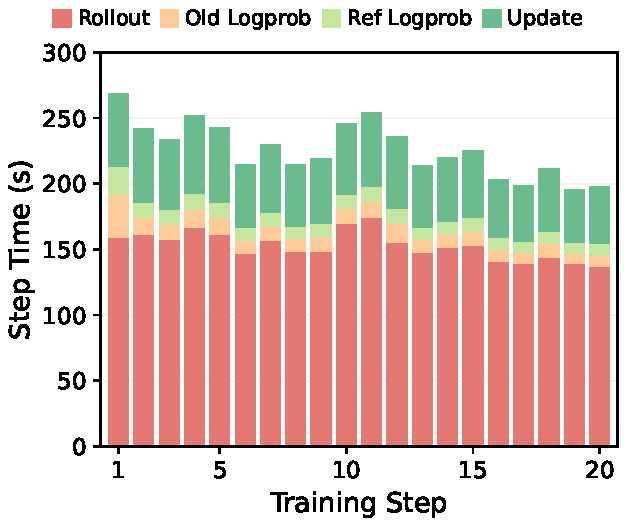
\includegraphics[width=\linewidth]{figures/main_rollout_step_time_llama8b.pdf}
        \caption{}
        \label{fig:rollout_llama_bottleneck_step}
    \end{subfigure}
    \hfill
    \begin{subfigure}[t]{0.32\linewidth}
        \centering
        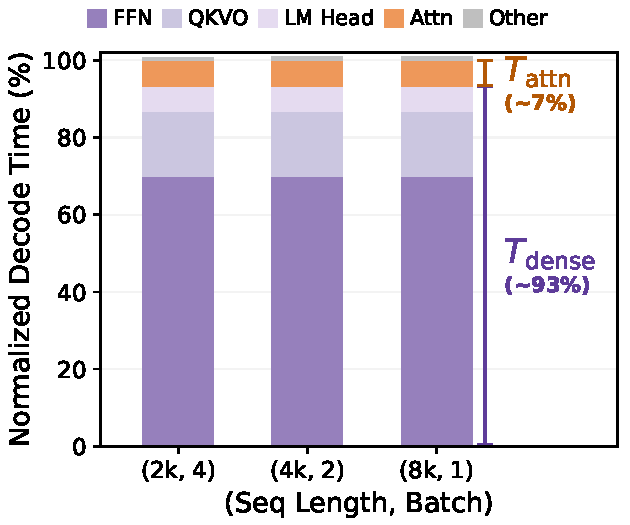
\includegraphics[width=\linewidth]{figures/main_rollout_decode_breakdown_llama_8b.pdf}
        \caption{}
        \label{fig:rollout_llama_decode_breakdown}
    \end{subfigure}
    \hfill
    \begin{subfigure}[t]{0.32\linewidth}
        \centering
        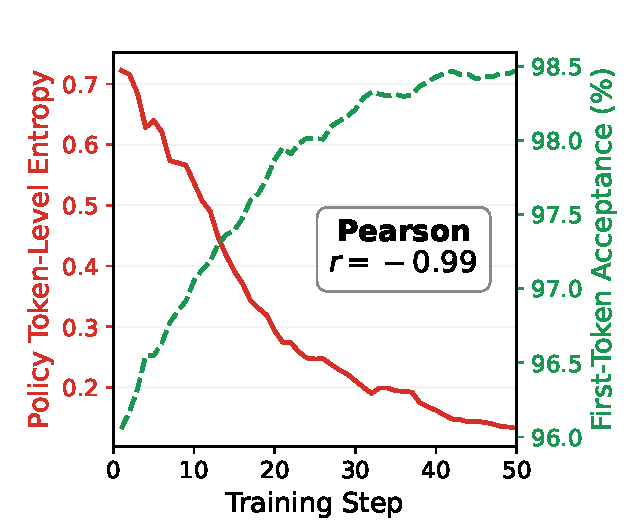
\includegraphics[width=\linewidth]{figures/main_motivation_entropy_acc_qwen7b.pdf}
        \caption{}
        \label{fig:entropy_acceptance_qwen}
    \end{subfigure}

    \caption{
    \textbf{Empirical characteristics of RL rollout decoding.}
    (a) Step-time decomposition over the first 20 training steps.
    (b) Single-token decode-time breakdown in RL rollout-tail phases.
    (c) Inverse correlation between target-policy entropy and quantized-drafter first-token acceptance over steps.
    }
    \label{fig:rollout_bottleneck}
\end{figure*}